\mfpicnumber{1}

\opengraphsfile{Sinusoid}

\setcounter{footnote}{0}

\label{Sinusoid}

In the same way exponential functions can be used to model a wide variety of phenomena in nature,\footnote{See Section \ref{ExpLogApplications}.} the cosine and sine functions can be used to model their fair share of natural behaviors. In section \ref{TrigGraphs}, we introduced the concept of a sinusoid as a function which can be written either in the form $C(x) = A \cos(\omega x + \phi) + B$ for $\omega > 0$ or equivalently, in the form $S(x) = A \sin(\omega x + \phi) + B$ for $\omega > 0$.  At the time, we remained undecided as to which form we preferred, but the time for such indecision is over.  For clarity of exposition we focus on the sine function\footnote{Sine haters can use the co-function identity $\cos\left(\frac{\pi}{2} - \theta\right) = \sin(\theta)$ to turn all of the sines into cosines.} in this section and switch to the independent variable $t$, since the applications in this section are time-dependent.  We reintroduce and summarize all of the important facts and definitions about this form of the sinusoid below.

\smallskip

\colorbox{ResultColor}{\bbm

\phantomsection
\label{sinesinusoidprops}

\centerline{\textbf{Properties of the Sinusoid \boldmath  $S(t) = A \sin(\omega t + \phi) + B$}} \index{sinusoid ! properties of}

\begin{itemize}

\item  The \textbf{amplitude}\index{sinusoid ! amplitude}\index{amplitude} is $|A|$

\item  The \textbf{angular frequency}\index{sinusoid ! frequency ! angular}\index{frequency ! angular} is $\omega$ and the \textbf{ordinary frequency}\index{sinusoid ! frequency ! ordinary}\index{frequency ! ordinary} is $f  = \dfrac{\omega}{2\pi}$

\item  The \textbf{period}\index{sinusoid ! period}\index{period ! of a sinusoid} is  $T = \dfrac{1}{f} = \dfrac{2\pi}{\omega}$

\item  The \textbf{phase}\index{sinusoid ! phase}\index{phase} is $\phi$ and the \textbf{phase shift}\index{sinusoid ! phase shift}\index{phase shift} is $-\dfrac{\phi}{\omega}$

\item  The \textbf{vertical shift}\index{sinusoid ! vertical shift}\index{sinusoid ! baseline} or \textbf{baseline} is $B$

\end{itemize}

\ebm}

\medskip

Along with knowing these formulas, it is helpful to remember what these quantities mean in context.  The amplitude measures the maximum displacement of the sine wave from its baseline (determined by the vertical shift), the period is the length of time it takes to complete one cycle of the sinusoid, the angular frequency tells how many cycles are completed over an interval of length $2\pi$, and the ordinary frequency measures how many cycles occur per unit of time. The phase indicates what angle $\phi$ corresponds to $t=0$, and the phase shift represents how much of a `head start' the sinusoid has over the un-shifted sine function.  The figure below is repeated from Section \ref{TrigGraphs}.

\begin{center}
\phantomsection
\label{genericsinsuoidfigure}\index{sinusoid ! graph of}
\begin{mfpic}[15]{-6.5}{6.5}{-6.5}{6.5}
\dashed \polyline{(-6.2832,0), (6.2832,0)}
\function{-6.2832, 6.2832, 0.1}{0-6*sin(x/2)}
\arrow \reverse \arrow \polyline{(-3.1416, 0.25), (-3.1416, 5.75)}
\gclear \tlabelrect[cc](-3.1416, 3){amplitude}
\gclear \tlabelrect[cc](3.1416, 0){baseline}
\arrow \reverse \arrow \polyline{(-6.2832,-6.5), (6.2832,-6.5)}
\gclear \tlabelrect[cc](0, -6.5){period}
\end{mfpic}

\end{center}


In Section \ref{circularmotion}, we introduced the concept of circular motion and in Section \ref{cosinesinebeyond}, we developed formulas for circular motion.  Our first foray into sinusoidal motion puts these notions to good use. 

\begin{ex} \label{ycoordonwheel} Recall from Exercise \ref{giantwheelmotion} in Section \ref{Angles} that The Giant Wheel at Cedar Point is a circle with diameter 128 feet which sits on an 8 foot tall platform making its overall height 136 feet.   It completes two revolutions in 2 minutes and 7 seconds.  Assuming that the riders are at the edge of the circle, find a sinusoid which describes the height of the passengers above the ground  $t$ seconds after they pass the point on the wheel closest to the ground.

{\bf Solution.}  We sketch the problem situation below and assume a counter-clockwise rotation.\footnote{Otherwise, we could just observe the motion of the wheel from the other side.} 

\begin{center}
\begin{mfpic}[20]{-5}{5}{-1}{9}
\polyline{(-5,0), (5,0)}
\polyline{(0,0), (0,1)}
\point[3pt]{(0,0), (0,1), (-3.46,3), (4,5)}
\plotsymbol[3pt]{Asterisk}{(0,5)}
\tlabel[cc](0,-0.5){\scriptsize $O$}
\tlabel[cc](0.5,0.5){\scriptsize $P$}
\tlabel[cc](4.5,5){\scriptsize $Q$}
\tlabel[cc](5,7){\scriptsize $\theta$}
\dashed \polyline{(5,5), (6,5)}
\arrow \reverse \arrow \polyline{(-3.46, 0.25),(-3.46, 2.75)}
\gclear \tlabelrect[cc](-3.46,1.5){\scriptsize $h$}
\shiftpath{(0,5)} \polyline{\plr{(0,0)}, \plr{(4,0)}}
\shiftpath{(0,5)} \polyline{\plr{(0,0)}, \plr{(4,15)}}
\shiftpath{(0,5)} \polyline{\plr{(0,0)}, \plr{(4,30)}}
\shiftpath{(0,5)} \polyline{\plr{(0,0)}, \plr{(4,45)}}
\shiftpath{(0,5)} \polyline{\plr{(0,0)}, \plr{(4,60)}}
\shiftpath{(0,5)} \polyline{\plr{(0,0)}, \plr{(4,75)}}
\shiftpath{(0,5)} \polyline{\plr{(0,0)}, \plr{(4,90)}}
\shiftpath{(0,5)} \polyline{\plr{(0,0)}, \plr{(4,105)}}
\shiftpath{(0,5)} \polyline{\plr{(0,0)}, \plr{(4,120)}}
\shiftpath{(0,5)} \polyline{\plr{(0,0)}, \plr{(4,135)}}
\shiftpath{(0,5)} \polyline{\plr{(0,0)}, \plr{(4,150)}}
\shiftpath{(0,5)} \polyline{\plr{(0,0)}, \plr{(4,165)}}
\shiftpath{(0,5)} \polyline{\plr{(0,0)}, \plr{(4,180)}}
\shiftpath{(0,5)} \polyline{\plr{(0,0)}, \plr{(4,195)}}
\shiftpath{(0,5)} \polyline{\plr{(0,0)}, \plr{(4,210)}}
\shiftpath{(0,5)} \polyline{\plr{(0,0)}, \plr{(4,225)}}
\shiftpath{(0,5)} \polyline{\plr{(0,0)}, \plr{(4,240)}}
\shiftpath{(0,5)} \polyline{\plr{(0,0)}, \plr{(4,255)}}
\shiftpath{(0,5)} \polyline{\plr{(0,0)}, \plr{(4,270)}}
\shiftpath{(0,5)} \polyline{\plr{(0,0)}, \plr{(4,285)}}
\shiftpath{(0,5)} \polyline{\plr{(0,0)}, \plr{(4,300)}}
\shiftpath{(0,5)} \polyline{\plr{(0,0)}, \plr{(4,315)}}
\shiftpath{(0,5)} \polyline{\plr{(0,0)}, \plr{(4,330)}}
\shiftpath{(0,5)} \polyline{\plr{(0,0)}, \plr{(4,345)}}
\arrow \shiftpath{(0,5)} \parafcn{-90, -80,5}{(4*cosd(t), 4*sind(t))}
\arrow \shiftpath{(0,5)} \parafcn{-80, 10,5}{(4*cosd(t), 4*sind(t))}
\arrow \shiftpath{(0,5)} \parafcn{10, 100,5}{(4*cosd(t), 4*sind(t))}
\arrow \shiftpath{(0,5)} \parafcn{100, 190,5}{(4*cosd(t), 4*sind(t))}
\shiftpath{(0,5)} \parafcn{190, 270,5}{(4*cosd(t), 4*sind(t))}
\arrow \shiftpath{(0,5)} \parafcn{5,50,5}{(5*cosd(t), 5*sind(t))}
\end{mfpic}
\end{center}

We know from the equations given on page \pageref{equationsforcircularmotion} in Section \ref{cosinesinebeyond} that the $y$-coordinate for counter-clockwise motion on a circle of radius $r$ centered at the origin with constant angular velocity (frequency) $\omega$ is given by $y = r\sin(\omega t)$.  Here,  $t=0$ corresponds to the point $(r,0)$ so that $\theta$, the angle measuring the amount of rotation, is in standard position. In our case, the diameter of the wheel is 128 feet, so the radius is $r = 64$ feet. Since the wheel completes two revolutions in 2 minutes and 7 seconds (which is $127$ seconds) the period $T = \frac{1}{2} (127) = \frac{127}{2}$ seconds.  Hence, the angular frequency is $\omega = \frac{2\pi}{T} = \frac{4 \pi}{127}$ radians per second.  Putting these two pieces of information together, we have that  $y = 64 \sin\left(\frac{4 \pi}{127} t\right)$ describes the $y$-coordinate on the Giant Wheel after $t$ seconds, assuming it is centered at $(0,0)$ with $t=0$ corresponding to the point $Q$.  In order to find an expression for $h$, we take the point $O$ in the figure as the origin.    Since the base of the Giant Wheel ride is $8$ feet above the ground and the Giant Wheel itself has a radius of  $64$ feet, its center is $72$ feet above the ground. To account for this vertical shift upward,\footnote{We are readjusting our `baseline' from $y=0$ to $y=72$.} we add $72$ to our formula for $y$ to obtain the new formula $h = y  + 72 = 64 \sin\left(\frac{4 \pi}{127} t\right) + 72$.  Next, we need to adjust things so that $t=0$ corresponds to the point $P$ instead of the point $Q$. This is where the phase comes into play.  Geometrically, we need to shift the angle $\theta$ in the figure back $\frac{\pi}{2}$ radians.  From Section \ref{cosinesinebeyond}, we know $\theta = \omega t = \frac{4 \pi}{127} t$, so we (temporarily) write the height in terms of $\theta$ as  $h =64 \sin\left(\theta\right) + 72$.    Subtracting $\frac{\pi}{2}$ from $\theta$ gives the final answer $h(t) = 64 \sin\left(\theta - \frac{\pi}{2}\right) + 72 = 64\sin\left(\frac{4 \pi}{127} t -\frac{\pi}{2} \right) + 72$. We can check the reasonableness of our answer by graphing $y = h(t)$ over the interval $\left[0, \frac{127}{2}\right]$.

\begin{center}

\begin{mfpic}[20][10]{-1}{7}{-1}{15}
\axes
\tlabel[cc](7,-0.5){\scriptsize $t$}
\tlabel[cc](0.5, 15){\scriptsize $y$}
\xmarks{6.35}
\ymarks{0.8, 7.2, 13.6}
\point[3pt]{(0,0.8), (1.59, 7.2), (3.18, 13.6), (4.76, 7.2), (6.35,0.8)}
\tlabelsep{5pt}
\scriptsize
\axislabels{x}{{$\frac{127}{2}$} 6.35}
\axislabels{y}{{$8$} 0.8, {$72$} 7.2, {$136$} 13.6}
\normalsize
\function{0,6.35,0.1}{6.4*(sin(.989*x - 1.57))+7.2}
\end{mfpic}

\end{center}

\vspace{-.5in} \qed

\end{ex}

A few remarks about Example \ref{ycoordonwheel} are in order.  First, note that the amplitude of $64$ in our answer corresponds to the radius of the Giant Wheel.  This means that passengers on the Giant Wheel never stray more than $64$ feet vertically from the center of the Wheel, which makes sense.  Second, the phase shift of our answer works out to be $\frac{\pi/2}{4\pi/127} = \frac{127}{8} = 15.875$.  This represents the `time delay' (in seconds) we introduce by starting the motion at the point $P$ as opposed to the point $Q$.  Said differently, passengers which `start' at $P$ take  $15.875$ seconds to `catch up' to the point $Q$.  

\medskip

Our next example revisits the daylight data first introduced in Section \ref{Regression}, Exercise \ref{regsunlight}.

\begin{ex} \label{sinusoidsunlight} According to the \href{http://aa.usno.navy.mil/data/docs/RS_OneYear.php}{\underline{U.S. Naval Observatory}} website, the number of hours $H$ of daylight that Fairbanks, Alaska received on the 21st day of the $n$th month of 2009 is given below.  Here  $t = 1$ represents January 21, 2009, $t = 2$ represents February 21, 2009, and so on.  

\medskip

\small

\noindent \begin{tabular}{|l|r|r|r|r|r|r|r|r|r|r|r|r|} \hline
Month  & & & & & & & & & & & & \\
Number & 1 & 2 & 3 & 4 & 5 & 6 & 7 & 8 & 9 & 10 & 11 & 12\\ 
\hline 
Hours of  & & & & & & & & & & & & \\
Daylight & 5.8 & 9.3 & 12.4 & 15.9 & 19.4 & 21.8 & 19.4 & 15.6 & 12.4 & 9.1 & 5.6 & 3.3 \\ \hline
\end{tabular}

\normalsize

\medskip

\begin{enumerate}

\item  \label{roughsinusoidfit} Find a sinusoid which models these data and use a graphing utility to graph your answer along with the data. 

\item   Compare your answer to part \ref{roughsinusoidfit} to one obtained using the regression feature of a calculator.

\end{enumerate}

{\bf Solution.}

\begin{enumerate}

\item  To get a feel for the data, we plot it below.

\begin{center}

\begin{mfpic}[15][7.5]{-1}{13}{-1}{23}

\axes
\xmarks{1,2,3,4,5,6,7,8,9,10,11,12}
\ymarks{2,4,6,8,10,12,14,16,18,20,22}
\tlabel[cc](13,-0.5){\scriptsize $t$}
\tlabel[cc](0.5,23){\scriptsize $H$}
\tlabelsep{5pt}
\scriptsize
\axislabels{x}{{$1$} 1, {$2$} 2, {$3$} 3, {$4$} 4, {$5$} 5, {$6$} 6, {$7$} 7, {$8$} 8, {$9$} 9, {$10$} 10, {$11$} 11, {$12$} 12}
\axislabels{y}{{$2$} 2, {$4$} 4, {$6$} 6, {$8$} 8, {$10$} 10, {$12$} 12, {$14$} 14, {$16$} 16, {$18$} 18, {$20$} 20, {$22$} 22}
\normalsize
\plotsymbol[3pt]{Square}{(1,5.8), (2,9.3), (3,12.4), (4, 15.9), (5, 19.4), (6,21.8), (7,19.4), (8,15.6), (9,12.4), (10,9.1), (11,5.6), (12, 3.3)}
\end{mfpic}

\end{center}

\vspace*{-.15in}

The data certainly appear sinusoidal,\footnote{Okay, it appears to be the `$\wedge$' shape we saw in some of the graphs in Section \ref{AbsoluteValueFunctions}.  Just humor us.} but when it comes down to it, fitting a sinusoid to data manually is not an exact science.  We do our best to find the constants $A$, $\omega$, $\phi$ and $B$ so that the function $H(t) = A\sin(\omega t + \phi) + B$ closely matches the data.  We first go after the vertical shift $B$ whose value determines the baseline.  In a typical sinusoid, the value of $B$ is the average of the maximum and minimum values.  So here we take $B = \frac{3.3+21.8}{2} = 12.55$.  Next is the amplitude $A$ which is the displacement from the baseline to the maximum (and minimum) values.  We find $A = 21.8 - 12.55 = 12.55 - 3.3 = 9.25$.  At this point, we have $H(t) = 9.25\sin(\omega t + \phi) + 12.55$.  Next, we go after the angular frequency $\omega$.  Since the data collected is over the span of a year (12 months), we take the period $T = 12$ months.\footnote{Even though the data collected lies in the interval $[1,12]$, which has a length of $11$, we need to think of the data point at $t=1$ as a representative sample of the amount of daylight for every day in January. That is, it represents $H(t)$ over the interval $[0,1]$.  Similarly, $t=2$ is a sample of $H(t)$ over $[1,2]$, and so forth.}   This means $\omega = \frac{2\pi}{T} = \frac{2\pi}{12} = \frac{\pi}{6}$.  The last quantity to find is the phase $\phi$. Unlike the previous example,  it is easier in this case to find the phase shift $-\frac{\phi}{\omega}$.  Since we picked $A > 0$, the phase shift corresponds to the first value of $t$ with $H(t) = 12.55$ (the baseline value).\footnote{See the figure on page \pageref{genericsinsuoidfigure}.}  Here, we choose $t = 3$, since its corresponding $H$ value of $12.4$ is closer to  $12.55$ than the next value, $15.9$, which corresponds to $t=4$.  Hence, $-\frac{\phi}{\omega} = 3$, so $\phi = -3 \omega = -3 \left(\frac{\pi}{6}\right) = -\frac{\pi}{2}$.  We have $H(t) = 9.25 \sin\left(\frac{\pi}{6} t - \frac{\pi}{2}\right) + 12.55$. Below is a graph of our data with the curve $y = H(t)$.

%\vspace{-.1in}

\begin{center}

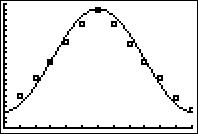
\includegraphics[width=1.8in]{./AppExtGraphics/Sinusoid01.jpg}

\end{center}

\item  Using the `SinReg' command, we graph the calculator's regression below.

%\vspace{-.25in}

\begin{center}

\begin{tabular}{ccc}


\includegraphics[width=1.8in]{./AppExtGraphics/Sinusoid02.jpg} &
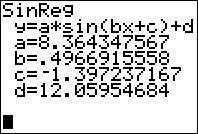
\includegraphics[width=1.8in]{./AppExtGraphics/Sinusoid03.jpg} & 
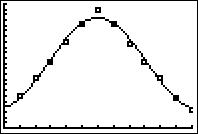
\includegraphics[width=1.8in]{./AppExtGraphics/Sinusoid04.jpg} \\


\end{tabular}
\end{center}

While both models seem to be reasonable fits to the data, the calculator model is possibly the better fit.  The calculator does not give us an $r^{2}$ value like it did for linear regressions in Section \ref{Regression}, nor does it give us an $R^{2}$ value like it did for quadratic, cubic and quartic regressions as in Section \ref{GraphsofPolynomials}.  The reason for this, much like the reason for the absence of $R^{2}$ for the logistic model in Section \ref{ExpLogApplications}, is beyond the scope of this course.  We'll just have to use our own good judgment when choosing the best sinusoid model.  \qed

\end{enumerate}

\end{ex}

\subsection{Harmonic Motion}
\label{harmomicmotion}

One of the major applications of sinusoids in Science and Engineering is the study of \index{harmonic motion} \textbf{harmonic motion}.   The equations for harmonic motion can be used to describe a wide range of phenomena, from the motion of an object on a spring, to the response of an electronic circuit.  In this subsection, we restrict our attention to modeling a simple spring system.  Before we jump into the Mathematics, there are some Physics terms and concepts we need to discuss.  In Physics, `mass' is defined as a measure of an object's resistance to straight-line motion whereas `weight' is the amount of force (pull) gravity exerts on an object.  An object's mass cannot change,\footnote{Well, assuming the object isn't subjected to relativistic speeds \dots} while its weight could change.  An object which weighs 6 pounds on the surface of the Earth would weigh 1 pound on the surface of the Moon, but its mass is the same in both places. In the English system of units, `pounds' (lbs.) is a measure of force (weight), and the corresponding unit of mass is the `slug'. In the SI system, the unit of force is `Newtons' (N) and the associated unit of mass is the `kilogram' (kg). We convert between mass and weight using the formula\footnote{This is a consequence of Newton's Second Law of Motion $F = ma$ where $F$ is force, $m$ is mass and $a$ is acceleration.  In our present setting, the force involved is weight which is caused by the acceleration due to gravity.} $w = mg$.   Here, $w$ is the weight of the object, $m$ is the mass and $g$ is the acceleration due to gravity.  In the English system, $g = 32 \frac{\text{feet}}{\text{second}^2}$, and in the SI system, $g = 9.8\frac{\text{meters}}{\text{second}^2}$. Hence, on Earth a \textit{mass} of 1 slug \textit{weighs} 32 lbs. and a \textit{mass} of 1 kg \textit{weighs} 9.8 N.\footnote{Note that $1$ pound $ = 1 \, \frac{\text{slug foot}}{\text{second}^2}$ and $1$ Newton $ = 1 \, \frac{\text{kg meter}}{\text{second}^2}$.}    Suppose we attach an object with mass $m$ to a spring as depicted below. The weight of the object will stretch the spring.   The system is said to be in `equilibrium' when the weight of the object is perfectly balanced with the restorative force of the spring.  How far the spring stretches to reach equilibrium depends on the spring's `spring constant'. Usually denoted by the letter $k$, the spring constant relates the force $F$ applied to the spring to the amount $d$ the spring stretches in accordance with \href{http://en.wikipedia.org/wiki/Hooke's_law}{\underline{Hooke's Law}}\footnote{Look familiar?  We saw Hooke's Law in Section \ref{Variation}.} $F = kd$.  If the object is released above or below the equilibrium position, or if the object is released with an upward or downward velocity, the object will bounce up and down on the end of the spring until some external force stops it.  If we let $x(t)$ denote the object's displacement from the equilibrium position at time $t$, then $x(t) = 0$ means the object is at the equilibrium position, $x(t) < 0$ means the object is \textit{above} the equilibrium position, and $x(t) > 0$ means the object is \textit{below} the equilibrium position.  The function $x(t)$ is called the `equation of motion' of the object.\footnote{To keep units compatible, if we are using the English system, we use feet (ft.) to measure displacement.  If we are in the SI system, we measure displacement in meters (m). Time is always measured in seconds (s).}

\begin{center}

\begin{tabular}[t]{ccc}

\begin{mfpic}[15]{-3}{3}{-2}{5}
\dashed \polyline{(-3,0.5), (3,0.5)}
\hatchcolor[gray]{.7}
\lhatch \rect{(-3,4), (3,5)}
\fillcolor[gray]{.7} 
\gfill \rect{(-0.5,0), (0.5,1)}
\polyline{(0,4), (0,3.5), (0.25,3.25), (-0.25, 3), (0.25,2.75), (-0.25,2.5), (0.25,2.25), (-0.25,2), (0.25,1.75), (-0.25,1.5), (0, 1.25), (0,1)}
\penwd{1.025}
\rect{(-3,4), (3,5)}
\rect{(-0.5,0), (0.5,1)}
\drawcolor{white} \polyline{(-3,-2), (-3,2)}
\end{mfpic} 

&

\hspace{0.5in}
\begin{mfpic}[15]{-3}{3}{-2}{5}
\dashed \polyline{(-3,0.5), (3,0.5)}
\hatchcolor[gray]{.7}
\lhatch \rect{(-3,4), (3,5)}
\fillcolor[gray]{.7} 
\gfill \rect{(-0.5,0.95), (0.5,1.95)}
\polyline{(0,4), (0,3.5), (0.25,3.4), (-0.25, 3.25), (0.25,3.1), (-0.25,2.95), (0.25,2.8), (-0.25,2.65), (0.25,2.5), (-0.25,2.35), (0, 2.2), (0,1.95)}
\penwd{1.025}
\rect{(-3,4), (3,5)}
\rect{(-0.5,0.95), (0.5,1.95)}
\drawcolor{white} \polyline{(-3,-2), (-3,2)}
\end{mfpic} 

&

\hspace{0.5in}
\begin{mfpic}[15]{-3}{3}{-2}{5}
\dashed \polyline{(-3,0.5), (3,0.5)}
\hatchcolor[gray]{.7}
\lhatch \rect{(-3,4), (3,5)}
\fillcolor[gray]{.7} 
\gfill \rect{(-0.5,-1.35), (0.5,-0.35)}
\polyline{(0,4), (0,3.5), (0.25,3.1), (-0.25, 2.7), (0.25,2.3), (-0.25, 1.9), (0.25,1.5), (-0.25,1.1), (0.25,0.7), (-0.25,0.3), (0, -0.1), (0,-0.35)}
\penwd{1.025}
\rect{(-3,4), (3,5)}
\rect{(-0.5,-1.35), (0.5,-0.35)}
\drawcolor{white} \polyline{(-3,-2), (-3,2)}
\end{mfpic} \\
 
$x(t) = 0$ at the &
\hspace{0.5in}
$x(t) < 0$ above the&
\hspace{0.5in}
$x(t) > 0$ below the \\

equilibrium position & 
\hspace{0.5in}
equilibrium position & 
\hspace{0.5in}
equilibrium position \\

\end{tabular}

\end{center}

If we ignore all other influences on the system except gravity and the spring force, then Physics tells us that gravity and the spring force will battle each other forever and the object will oscillate indefinitely.  In this case, we describe the motion as `free' (meaning there is no external force causing the motion) and `undamped' (meaning we ignore friction caused by surrounding medium, which in our case is air).  The following theorem, which comes from Differential Equations, gives $x(t)$ as a function of the mass $m$ of the object, the spring constant $k$, the initial displacement $x_{\text{\tiny $0$}}$ of the object and initial velocity $v_{\text{\tiny $0$}}$ of the object.  As with $x(t)$, $x_{\text{\tiny $0$}} = 0$ means the object is released from the equilibrium position, $x_{\text{\tiny $0$}} < 0$ means the object is released \textit{above} the equilibrium position and $x_{\text{\tiny $0$}}>0$ means the object is released \textit{below} the equilibrium position.  As far as the initial velocity $v_{\text{\tiny $0$}}$ is concerned, $v_{\text{\tiny $0$}} =0 $ means the object is released `from rest,' $v_{\text{\tiny $0$}}<0$ means the object is heading \textit{upwards} and $v_{\text{\tiny $0$}}>0$ means the object is heading \textit{downwards}.\footnote{The sign conventions here are carried over from Physics.  If not for the spring, the object would fall towards the ground, which is the `natural' or `positive' direction.  Since the spring force acts in direct opposition to gravity,  any movement upwards is considered `negative'.}

\medskip

\colorbox{ResultColor}{\bbm
\begin{thm} \label{freeundampedmotion} \textbf{Equation for Free Undamped Harmonic Motion:}  Suppose an object of  mass $m$ is suspended from a spring with spring constant $k$.  If the initial displacement from the equilibrium position is $x_{\text{\tiny $0$}}$ and the initial velocity of the object is $v_{\text{\tiny $0$}}$, then the displacement $x$ from the equilibrium position at time $t$ is given by  $x(t) = A \sin(\omega t + \phi)$ where

\begin{itemize}

\item  $\omega = \sqrt{\dfrac{k}{m}}$ and $A = \sqrt{x_{\text{\tiny $0$}}^2 + \left( \dfrac{v_{\text{\tiny $0$}}}{\omega}\right)^2}$

\item $A\sin(\phi) = x_{\text{\tiny $0$}}$ and $A\omega\cos(\phi) = v_{\text{\tiny $0$}}$.

\end{itemize} 

\end{thm}

\ebm}

\medskip

It is a great exercise in `dimensional analysis' to verify that the formulas given in Theorem \ref{freeundampedmotion} work out so that $\omega$ has units $\frac{1}{s}$ and  $A$ has units ft. or m, depending on which system we choose.

\begin{ex} \label{freeudampedex}  Suppose an object weighing  64 pounds stretches a spring 8 feet.  

\begin{enumerate}

\item  If the object is attached to the spring and released 3 feet below the equilibrium position from rest, find the equation of motion of the object, $x(t)$.  When does the object first pass through the equilibrium position?  Is the object heading upwards or downwards at this instant? 

\item  If the object is attached to the spring and released 3 feet below the equilibrium position with an upward velocity of $8$ feet  per second, find the equation of motion of the object, $x(t)$.  What is the longest distance the object travels \textit{above} the equilibrium position?  When does this first happen? Confirm your result using a graphing utility.

\end{enumerate}

{\bf Solution.} In order to use the formulas in Theorem \ref{freeundampedmotion}, we first need to determine the spring constant $k$ and the mass of the object $m$.  To find $k$, we use Hooke's Law $F = kd$.  We know the object weighs $64$ lbs. and stretches the spring $8$ ft.. Using $F = 64$ and $d = 8$,  we get  $64  = k \cdot 8 $, or  $k = 8 \frac{\text{lbs.}}{\text{ft.}}$.  To find $m$, we use $w = mg$ with $w = 64$ lbs. and $g =32 \frac{\text{ft.}}{s^2}$.  We get $m = 2$ slugs.  We can now proceed to apply Theorem \ref{freeundampedmotion}.

\begin{enumerate}

\item  With $k = 8$ and $m = 2$, we get $\omega = \sqrt{\frac{k}{m}} = \sqrt{\frac{8}{2}} = 2$. We are told that the object is released 3 feet \textit{below} the equilibrium position `from rest.'  This means  $x_{\text{\tiny $0$}} = 3$ and  $v_{\text{\tiny $0$}} = 0$.  Therefore, $A = \sqrt{x_{\text{\tiny $0$}}^2 + \left( \frac{v_{\text{\tiny $0$}}}{\omega}\right)^2} = \sqrt{3^2 + 0^2} = 3$.  To determine the phase $\phi$, we have $A\sin(\phi) = x_{\text{\tiny $0$}}$, which in this case gives $3 \sin(\phi) = 3$ so $\sin(\phi) = 1$.  Only $\phi = \frac{\pi}{2}$ and angles coterminal to it satisfy this condition, so we pick\footnote{For confirmation, we note that $A\omega\cos(\phi) = v_{\text{\tiny $0$}}$, which in this case reduces to $6\cos(\phi) = 0$.} the phase to be $\phi = \frac{\pi}{2}$.  Hence, the equation of motion is $x(t) = 3\sin\left(2t + \frac{\pi}{2}\right)$.  To find when the object passes through the equilibrium position we solve $x(t)= 3\sin\left(2t + \frac{\pi}{2}\right) = 0$. Going through the usual analysis we find $t = -\frac{\pi}{4} + \frac{\pi}{2} k$ for integers $k$. Since we are interested in the first time the object passes through the equilibrium position, we look for the smallest positive $t$ value which in this case is $t = \frac{\pi}{4} \approx 0.78$ seconds after the  start of the motion.  Common sense suggests that if we release the object below the equilibrium position, the object should be traveling upwards when it first passes through it.  To check this answer, we graph one cycle of  $x(t)$.  Since our applied domain in this situation is $t \geq 0$, and the period of $x(t)$ is $T = \frac{2\pi}{\omega} = \frac{2\pi}{2} = \pi$, we graph $x(t)$ over the interval $[0,\pi]$.  Remembering that $x(t) > 0$ means the object is below the equilibrium position and $x(t) < 0$ means the object is above the equilibrium position, the fact our graph is crossing through the $t$-axis from positive $x$ to negative $x$ at $t = \frac{\pi}{4}$ confirms our answer.

\item  The only difference between this problem and the previous problem is that we now release the object with an upward velocity of $8 \, \frac{\text{ft}}{s}$.  We still have $\omega = 2$ and $x_{\text{\tiny $0$}} = 3$, but now we have $v_{\text{\tiny $0$}} = -8$, the negative indicating the velocity is directed upwards. Here, we get $A = \sqrt{x_{\text{\tiny $0$}}^2 + \left( \frac{v_{\text{\tiny $0$}}}{\omega}\right)^2} = \sqrt{3^2 + (-4)^2} = 5$.  From $A\sin(\phi) = x_{\text{\tiny $0$}}$, we get $5\sin(\phi) = 3$ which gives $\sin(\phi) = \frac{3}{5}$.  From  $A\omega\cos(\phi) = v_{\text{\tiny $0$}}$, we get $10\cos(\phi) = -8$, or $\cos(\phi) = -\frac{4}{5}$.  This means that $\phi$ is a Quadrant II angle which we can describe in terms of either arcsine or arccosine.  Since $x(t)$ is expressed in terms of sine, we choose to express $\phi = \pi - \arcsin\left(\frac{3}{5}\right)$.  Hence, $x(t)= 5 \sin\left(2t + \left[\pi - \arcsin\left(\frac{3}{5}\right)\right]\right)$.  Since the amplitude of $x(t)$ is $5$, the object will travel at most $5$ feet above the equilibrium position.  To find when this happens, we solve the equation $x(t)= 5 \sin\left(2t + \left[\pi - \arcsin\left(\frac{3}{5}\right)\right]\right)= -5$, the negative once again signifying that the object is \textit{above} the equilibrium position.  Going through the usual machinations, we get $t = \frac{1}{2} \arcsin\left(\frac{3}{5}\right) +\frac{\pi}{4}  + \pi k$ for integers $k$. The smallest of these values occurs when $k=0$, that is, $t = \frac{1}{2} \arcsin\left(\frac{3}{5}\right) +\frac{\pi}{4} \approx 1.107$ seconds after the start of the motion. To check our answer using the calculator, we graph $y = 5 \sin\left(2x + \left[\pi - \arcsin\left(\frac{3}{5}\right)\right]\right)$ on a graphing utility and confirm the coordinates of the first relative minimum to be approximately $(1.107,-5)$.
\enlargethispage{\baselineskip}
\begin{center}

\begin{tabular}{cc}
\begin{mfpic}[20][15]{-0.5}{4}{-3.25}{3.5}

\axes
\point[3pt]{(0,3), (0.78,0), (1.57,-3), (2.36,0), (3.14,3)}
\tlabel[cc](4,-0.5){\scriptsize $t$}
\tlabel[cc](0.5,3.5){\scriptsize $x$}
\xmarks{0.78, 1.57, 2.36, 3.14}
\ymarks{-3,-2,-1,1,2,3}
\tlabelsep{5pt}
\scriptsize
\axislabels{x}{{$\frac{\pi}{4}\hspace{7pt}$} 0.78, {$\frac{\pi}{2}$} 1.57,{$\frac{3\pi}{4}$} 2.36, {$\pi$} 3.14}
\axislabels{y}{{$-3$} -3, {$-2$} -2,{$-1$} -1, {$1$} 1,{$2$} 2,{$3$} 3}
\normalsize
\arrow \function{0, 0.65, 0.1}{3*sin(2*x+1.57)}
\arrow \function{0.65, 1, 0.1}{3*sin(2*x+1.57)}
\function{1, 3.14, 0.1}{3*sin(2*x+1.57)}

\end{mfpic} &
\hspace{0.75in} 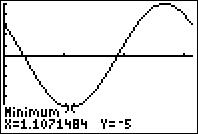
\includegraphics[width=2in]{./AppExtGraphics/Sinusoid05.jpg}\\

 $x(t)= 3\sin\left(2t + \frac{\pi}{2}\right)$ &
\hspace{0.75in} $y = 5 \sin\left(2x + \left[\pi - \arcsin\left(\frac{3}{5}\right)\right]\right)$ 


\end{tabular}

\end{center}

\qed

\end{enumerate}
\end{ex}

It is possible, though beyond the scope of this course, to model the effects of friction and other external forces acting on the system.\footnote{Take a good Differential Equations class to see this!}  While we may not have the Physics and Calculus background to \textit{derive} equations of motion for these scenarios, we can certainly analyze them.  We examine three cases in the following example.

\begin{ex} \label{underdampedresonance}  $~$  

\begin{enumerate}

\item  Write $x(t) = 5e^{-t/5} \cos(t) + 5e^{-t/5} \sqrt{3} \sin(t)$ in the form $x(t) = A(t) \sin(\omega t + \phi)$.  Graph $x(t)$ using a graphing utility.

\item  Write $x(t) = (t+3)\sqrt{2} \cos(2t) + (t+3) \sqrt{2} \sin(2t)$ in the form $x(t) = A(t) \sin(\omega t + \phi)$.  Graph $x(t)$  using a graphing utility.

\item  Find the period of $x(t) = 5\sin(6t) - 5\sin\left(8t\right)$.  Graph $x(t)$ using a graphing utility.

\end{enumerate}

{\bf Solution.}

\begin{enumerate}

\item  We start rewriting  $x(t) = 5e^{-t/5} \cos(t) + 5e^{-t/5} \sqrt{3} \sin(t)$ by factoring out   $5e^{-t/5}$ from both terms to get  $x(t) = 5e^{-t/5} \left( \cos(t) + \sqrt{3} \sin(t)\right)$. We convert what's left in parentheses to the required form using the formulas introduced in Exercise  \ref{sinusoidexercise2} from Section \ref{TrigGraphs}.  We find $\left( \cos(t) + \sqrt{3} \sin(t)\right) = 2\sin\left(t+\frac{\pi}{3}\right)$ so that $x(t) = 10e^{-t/5} \sin\left(t + \frac{\pi}{3}\right)$.  Graphing this on the calculator as $y = 10e^{-x/5} \sin\left(x + \frac{\pi}{3}\right)$ reveals some interesting behavior.  The sinusoidal nature continues indefinitely, but it is being attenuated.  In the sinusoid $A \sin(\omega x + \phi)$, the coefficient $A$ of the sine function is the amplitude.  In the case of $y = 10e^{-x/5} \sin\left(x + \frac{\pi}{3}\right)$, we can think of the \textit{function} $A(x) = 10e^{-x/5}$ as the amplitude.  As $x \rightarrow \infty$, $10e^{-x/5} \rightarrow 0$ which means the amplitude continues to shrink towards zero.  Indeed, if we graph $y = \pm 10e^{-x/5}$ along with $y = 10e^{-x/5} \sin\left(x + \frac{\pi}{3}\right)$, we see this attenuation taking place.  This equation corresponds to the motion of an object on a spring where there is a slight force which acts to `damp', or slow the motion.  An example of this kind of force would be the friction of the object against the air. In this model, the object oscillates forever, but with smaller and smaller amplitude. 
\begin{center}

\begin{tabular}{cc}

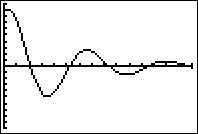
\includegraphics[width=2in]{./AppExtGraphics/Sinusoid06.jpg} &
\hspace{0.25in} 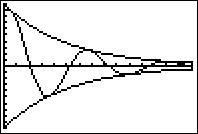
\includegraphics[width=2in]{./AppExtGraphics/Sinusoid07.jpg}  \\
 $y = 10e^{-x/5} \sin\left(x + \frac{\pi}{3}\right)$ &
\hspace{0.25in}  $y = 10e^{-x/5} \sin\left(x + \frac{\pi}{3}\right)$, $y = \pm 10e^{-x/5}$ \\

\end{tabular}
\end{center}

\item  Proceeding as in the first example, we factor out $(t+3)\sqrt{2}$ from each term in the function $x(t) = (t+3)\sqrt{2} \cos(2t) + (t+3) \sqrt{2} \sin(2t)$ to get $x(t) = (t+3)\sqrt{2}(\cos(2t) + \sin(2t))$.   We find $(\cos(2t) + \sin(2t)) = \sqrt{2} \sin\left(2t + \frac{\pi}{4}\right)$, so $x(t) = 2(t+3) \sin\left(2t + \frac{\pi}{4}\right)$.  Graphing this on the calculator as $y = 2(x+3) \sin\left(2x + \frac{\pi}{4}\right)$, we find the sinusoid's amplitude growing.  Since our amplitude function here is $A(x) = 2(x+3) = 2x+6$, which continues to grow without bound as $x \rightarrow \infty$, this is hardly surprising.  The phenomenon illustrated here is `forced' motion.  That is, we imagine that the entire apparatus on which the spring is attached is oscillating as well.  In this case, we are witnessing a `resonance' effect -- the frequency of the external oscillation matches the frequency of the motion of the object on the spring.\footnote{The reader is invited to investigate the destructive implications of \href{http://en.wikipedia.org/wiki/Resonance}{\underline{resonance}}.}


\begin{center}

\hspace{.1in} \begin{tabular}{cc}

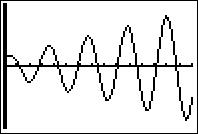
\includegraphics[width=2in]{./AppExtGraphics/Sinusoid08.jpg} &
\hspace{0.6in}  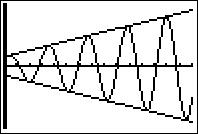
\includegraphics[width=2in]{./AppExtGraphics/Sinusoid09.jpg}  \\
$y = 2(x+3) \sin\left(2x + \frac{\pi}{4}\right)$ & 
\hspace{0.6in}  $y = 2(x+3) \sin\left(2x + \frac{\pi}{4}\right)$ \\
 & \hspace{0.6in}  $y = \pm 2(x+3)$ \\

\end{tabular}

\end{center}

\vspace{-.1in}

\item Last, but not least, we come to  $x(t) = 5\sin(6t) - 5\sin(8t)$.  To find the period of this function, we need to determine the length of the smallest interval on which both $f(t) = 5\sin(6t)$ and $g(t) = 5\sin(8t)$ complete a whole number of cycles.  To do this, we take the ratio of their frequencies and reduce to lowest terms:  $\frac{6}{8} = \frac{3}{4}$.  This tells us that for every $3$ cycles $f$ makes, $g$ makes $4$. In other words, the period of $x(t)$ is three times the period of $f(t)$ (which is four times the period of $g(t)$), or $\pi$.  We graph $y = 5\sin(6x) - 5\sin(8x)$ over $[0,\pi]$ on the calculator to check this.  This equation of motion also results from `forced' motion, but here the frequency of the external oscillation is different than that of the object on the spring.  Since the sinusoids here have different frequencies, they are `out of sync' and  do not amplify each other as in the previous example.  Taking things a step further, we can use a sum to product identity to rewrite $x(t) = 5\sin(6t) - 5\sin(8t)$ as $x(t) = -10 \sin(t) \cos(7t)$.  The lower frequency factor in this expression,  $-10\sin(t)$, plays an interesting role in the graph of $x(t)$.  Below we graph $y = 5\sin(6x) - 5\sin(8x)$ and $y = \pm 10 \sin(x)$ over $[0,2\pi]$.  This is an example of the `beat' phenomena, and the curious reader is invited to explore this concept as well.\footnote{A good place to start is this article on \href{http://en.wikipedia.org/wiki/Beat_(acoustics)}{\underline{beats}}.}

\enlargethispage{.2in}

\begin{center}

\begin{tabular}{cc}

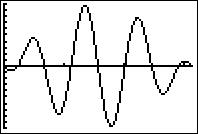
\includegraphics[width=2in]{./AppExtGraphics/Sinusoid10.jpg} &
\hspace{0.5in} 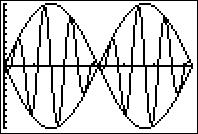
\includegraphics[width=2in]{./AppExtGraphics/Sinusoid11.jpg}  \\
$y = 5\sin(6x) - 5\sin(8x)$ over $[0,\pi]$ & 
\hspace{0.5in} $y = 5\sin(6x) - 5\sin(8x)$ and \\
 & \hspace{0.5in} $y = \pm 10 \sin(x)$ over $[0,2\pi]$\\

\end{tabular}

\end{center}

\end{enumerate}

\end{ex}

\vspace{-.35in} \qed

\newpage

\subsection{Exercises}

\begin{enumerate}

\item  The sounds we hear are made up of mechanical waves.  The note `A' above the note `middle C' is a sound wave with ordinary frequency $f = 440$ Hertz $= 440 \frac{\text{cycles}}{\text{second}}$.  Find a sinusoid which models this note, assuming that the amplitude is $1$ and the phase shift is $0$.

\item The voltage $V$ in an alternating current source has amplitude $220 \sqrt{2}$ and ordinary frequency $f = 60$ Hertz.  Find a sinusoid which models this voltage.  Assume that the phase is $0$.


\item \label{heightlondoneye} The \href{http://en.wikipedia.org/wiki/London_Eye}{\underline{London Eye}} is a popular tourist attraction in London, England and is one of the largest Ferris Wheels in the world.  It has a diameter of 135 meters and makes one revolution (counter-clockwise) every 30 minutes.  It is constructed so that the lowest part of the Eye reaches ground level, enabling passengers to simply walk on to, and off of, the ride.  Find a sinsuoid which models the height $h$ of the passenger above the ground in meters $t$ minutes after they board the Eye at ground level.

\item \label{leftrightlondoneye} On page \pageref{equationsforcircularmotion} in Section \ref{cosinesinebeyond}, we found the $x$-coordinate of counter-clockwise motion on a circle of radius $r$ with angular frequency $\omega$ to be $x = r\cos(\omega t)$, where $t=0$ corresponds to the point $(r,0)$.  Suppose we are in the situation of Exercise \ref{heightlondoneye} above.  Find a sinsusoid which models the horizontal \textit{displacement} $x$ of the passenger from the center of the Eye in meters $t$ minutes after they board the Eye.  Here we take $x(t) > 0$ to mean the passenger is to the \textit{right} of the center, while $x(t) < 0$ means the passenger is to the \textit{left} of the center.

\item  In Exercise \ref{yoyotrick} in Section \ref{Angles}, we introduced the yo-yo trick `Around the World' in which a yo-yo is thrown so it sweeps out a vertical circle.  As in that exercise, suppose the yo-yo string is 28 inches and it completes one revolution in 3 seconds.  If the closest the yo-yo ever gets to the ground is 2 inches, find a sinsuoid which models the height $h$ of the yo-yo above the ground in inches $t$ seconds after it leaves its lowest point.


\item  Suppose an object weighing $10$ pounds is suspended from the ceiling by a spring which stretches $2$ feet to its equilibrium position when the object is attached.  

\begin{enumerate}

\item  Find the spring constant $k$ in $\frac{\text{lbs.}}{\text{ft.}}$ and the mass of the object in slugs.
\item  Find the equation of motion of the object if it is released from $1$ foot \textit{below} the equilibrium position from rest.  When is the first time the object passes through the equilibrium position? In which direction is it heading?
\item  Find the equation of motion of the object if it is released from $6$ inches \textit{above} the equilibrium position with a \textit{downward} velocity of $2$ feet per second.  Find when the object passes through the equilibrium position heading downwards for the third time.


\end{enumerate}

\newpage

\item  Consider the pendulum below.  Ignoring air resistance, the angular displacement of the pendulum from the vertical position, $\theta$, can be modeled as a sinusoid.\footnote{Provided $\theta$ is kept `small.'  Carl remembers the `Rule of Thumb' as being $20^{\circ}$ or less.  Check with your friendly neighborhood physicist to make sure.}


\begin{center}

\begin{mfpic}[15]{-3}{3}{-5}{1}
\polyline{(0,0), (0,-5)}
\dashed \polyline{(0,0), (2.5, -4.33)}
\arrow \parafcn{275, 295, 5}{4*dir(t)}
\tlabel[cc](1.29, -4.83){$\theta$}
\hatchcolor[gray]{.7}
\lhatch \rect{(-3,0), (3,1)}
\fillcolor[gray]{.7} 
\gfill \circle{(0,-5),0.25}
\gfill \circle{(2.5, -4.33),0.20}
\penwd{1.025}
\circle{(0,-5),0.25}
\circle{(2.5, -4.33),0.25}
\rect{(-3,0), (3,1)}
\end{mfpic} 
\end{center}

The amplitude of the sinusoid is the same as the initial angular displacement, $\theta_{\text{\tiny $0$}}$, of the pendulum and the  period of the motion is given by

\[T = 2\pi \sqrt{\dfrac{l}{g}}\]

where $l$ is the length of the pendulum and $g$ is the acceleration due to gravity.

\begin{enumerate}

\item  Find a sinusoid which gives the angular displacement $\theta$ as a function of time, $t$. Arrange things so $\theta(0) = \theta_{\text{\tiny $0$}}$.

\item  In Exercise \ref{pendulumproblem} section \ref{AlgebraicFunctions}, you found the length of the pendulum needed in Jeff's antique Seth-Thomas clock to ensure the period of the pendulum is $\frac{1}{2}$ of a second. Assuming the initial displacement of the pendulum is $15^{\circ}$, find a sinusoid which models the displacement of the pendulum $\theta$ as a function of time, $t$, in seconds. 

\end{enumerate}


\item  The table below lists the average temperature of Lake Erie as measured in Cleveland, Ohio on the first of the month for each month during the years 1971 -- 2000.\footnote{See this website: \href{http://www.erh.noaa.gov/cle/climate/cle/normals/laketempcle.html}{\underline{http://www.erh.noaa.gov/cle/climate/cle/normals/laketempcle.html}.}}  For example,   $t=3$ represents the average of the temperatures recorded for Lake Erie on every March 1 for the years 1971 through 2000.

\medskip

\small

\noindent \begin{tabular}{|l|r|r|r|r|r|r|r|r|r|r|r|r|} \hline
Month  & & & & & & & & & & & & \\
Number, $t$ & 1 & 2 & 3 & 4 & 5 & 6 & 7 & 8 & 9 & 10 & 11 & 12\\ 
\hline 
Temperature  & & & & & & & & & & & & \\
($^{\circ}$ F), $T$ & 36 & 33 & 34 & 38 & 47 & 57 & 67 & 74 & 73 & 67 & 56 & 46 \\ \hline
\end{tabular}

\normalsize

\medskip

\begin{enumerate}

\item \label{LakeErieTempData} Using the techniques discussed in Example \ref{sinusoidsunlight}, fit a sinusoid to these data. 

\item  Using a graphing utility, graph your model along with the data set to judge the reasonableness of the fit.

\item Use the model you found in part \ref{LakeErieTempData} to predict the average temperature recorded for Lake Erie on April $15^{\text{th}}$ and September $15^{\text{th}}$ during the years 1971--2000.\footnote{The computed average is $41^{\circ}$F for April $15^{\text{th}}$ and $71^{\circ}$F for September $15^{\text{th}}$.}

\item Compare your results to those obtained using a graphing utility.

\end{enumerate}

\item  The fraction of the moon illuminated at midnight Eastern Standard Time on the $t^{\text{th}}$ day of June, 2009 is given in the table below.\footnote{See this website: \href{http://www.usno.navy.mil/USNO/astronomical-applications/data-services/frac-moon-ill}{\underline{http://www.usno.navy.mil/USNO/astronomical-applications/data-services/frac-moon-ill}.}} 


\medskip

\small

\noindent \begin{tabular}{|l|r|r|r|r|r|r|r|r|r|r|} \hline
Day of  & & & & & & & & & & \\
June, $t$ & 3 & 6 & 9 & 12 & 15 & 18 & 21 & 24 & 27 & 30\\ 
\hline 
Fraction  & & & & & & & & & & \\
Illuminated, $F$ & 0.81 & 0.98 & 0.98 & 0.83 & 0.57 & 0.27 & 0.04 & 0.03 & 0.26 & 0.58  \\ \hline
\end{tabular}

\normalsize

\medskip

\begin{enumerate}

\item \label{MoonIllumination} Using the techniques discussed in Example \ref{sinusoidsunlight}, fit a sinusoid to these data.\footnote{You may want to plot the data before you find the phase shift.} 

\item  Using a graphing utility, graph your model along with the data set to judge the reasonableness of the fit.

\item Use the model you found in part \ref{MoonIllumination} to predict the fraction of the moon illuminated on June 1, 2009. \footnote{The listed fraction is $0.62$.}

\item Compare your results to those obtained using a graphing utility.

\end{enumerate}

\item  With the help of your classmates, research the phenomena mentioned in Example \ref{underdampedresonance}, namely \href{http://en.wikipedia.org/wiki/Resonance}{\underline{resonance}} and \href{http://en.wikipedia.org/wiki/Beat_(acoustics)}{\underline{beats}}.

\item  With the help of your classmates, research \href{http://en.wikipedia.org/wiki/Amplitude_modulation}{\underline{Amplitude Modulation}} and \href{http://en.wikipedia.org/wiki/Frequency_modulation}{\underline{Frequency Modulation}}.

\item What other things in the world might be roughly sinusoidal?  Look to see what models you can find for them and share your results with your class.

\end{enumerate}

\newpage

\subsection{Answers}

\begin{enumerate}

\begin{multicols}{2}

\item  $S(t) = \sin\left(880\pi t\right)$

\item  $V(t) = 220 \sqrt{2} \sin\left(120\pi t\right)$

\end{multicols}


\begin{multicols}{2}

\item  $h(t) = 67.5 \sin\left(\frac{\pi}{15} t - \frac{\pi}{2} \right) + 67.5$

\item  $x(t) = 67.5 \cos\left(\frac{\pi}{15} t - \frac{\pi}{2} \right) = 67.5 \sin\left(\frac{\pi}{15} t \right)$

\end{multicols}

\item  $h(t) = 28\sin\left(\frac{2\pi}{3} t - \frac{\pi}{2}\right) + 30$

\item  \begin{enumerate} \item $k = 5 \, \frac{\text{lbs.}}{\text{ft.}}$ and $m = \frac{5}{16} \, \text{slugs}$

\item  $x(t) = \sin\left(4t + \frac{\pi}{2}\right)$.  The object first passes through the equilibrium point when $t = \frac{\pi}{8} \approx 0.39$ seconds after the motion starts.  At this time, the object is heading upwards.

\item  $x(t) = \frac{\sqrt{2}}{2} \sin\left(4t + \frac{7\pi}{4}\right)$.  The object passes through the equilibrium point heading downwards for the third time when $t = \frac{17\pi}{16} \approx 3.34$ seconds.


\end{enumerate}

\item  \begin{multicols}{2}

\begin{enumerate}

\item  $\theta(t) = \theta_{\text{\tiny $0$}} \sin\left(\sqrt{\frac{g}{l}}\, t + \frac{\pi}{2}\right)$

\item  $\theta(t) = \frac{\pi}{12} \sin\left(4\pi t + \frac{\pi}{2}\right)$
\end{enumerate}
\end{multicols}

\item  \begin{enumerate} \item  $T(t) = 20.5 \sin\left(\frac{\pi}{6} t - \pi\right) + 53.5$ 

\item  Our function and the data set are graphed below.  The sinusoid seems to be shifted to the right of our data.

\begin{center}

 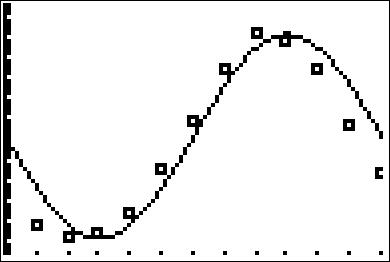
\includegraphics[width=2in]{./AppExtGraphics/Sinusoid12.jpg} 

\end{center}

\item The average temperature on April $15^{\text{th}}$ is approximately $T(4.5) \approx 39.00^{\circ}$F and the average temperature on September $15^{\text{th}}$ is approximately $T(9.5) \approx 73.38^{\circ}$F.

\item  Using a graphing calculator, we get the following

\begin{center}

\begin{tabular}{cc}

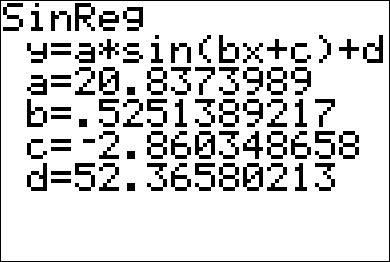
\includegraphics[width=2in]{./AppExtGraphics/Sinusoid13.jpg} &
\hspace{0.75in}  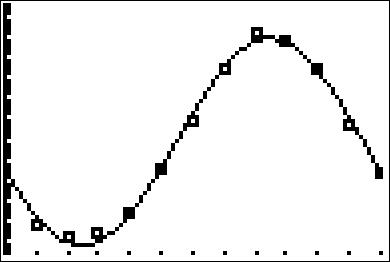
\includegraphics[width=2in]{./AppExtGraphics/Sinusoid14.jpg}  \\

\end{tabular}

\end{center}

This model predicts the average temperature for April $15^{\text{th}}$ to be approximately $42.43^{\circ}$F and the average temperature on September $15^{\text{th}}$ to be approximately $70.05^{\circ}$F.  This model appears to be more accurate.

\end{enumerate}


\item  \begin{enumerate} \item  Based on the shape of the data, we either choose $A<0$ or we find the \textit{second} value of $t$ which closely approximates the `baseline' value, $F = 0.505$.  We choose the latter to obtain $F(t) = 0.475 \sin\left(\frac{\pi}{15} t - 2\pi \right) + 0.505 =  0.475 \sin\left(\frac{\pi}{15} t\right) + 0.505$ 

\enlargethispage{\baselineskip}

\item  Our function and the data set are graphed below.  It's a pretty good fit.

\begin{center}

 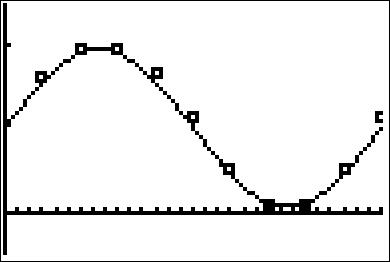
\includegraphics[width=2in]{./AppExtGraphics/Sinusoid15.jpg} 
 
 \end{center}

\item  The fraction of the moon illuminated on June 1st, 2009 is approximately $F(1) \approx 0.60$


\item  Using a graphing calculator, we get the following.

\begin{center}

\begin{tabular}{cc}

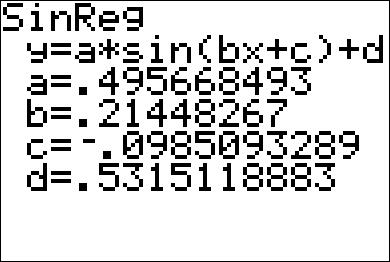
\includegraphics[width=2in]{./AppExtGraphics/Sinusoid16.jpg} &
\hspace{0.75in}  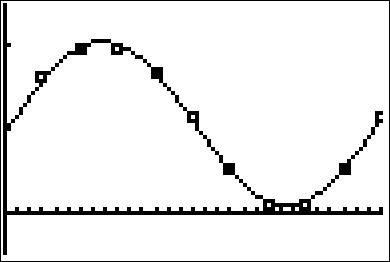
\includegraphics[width=2in]{./AppExtGraphics/Sinusoid17.jpg}  \\

\end{tabular}

\end{center}

This model predicts that the fraction of the moon illuminated on June 1st, 2009 is approximately $0.59$.  This appears to be a better fit to the data than our first model.

\end{enumerate}


\end{enumerate}

\closegraphsfile